\begin{figure}[hbt!]
	\caption{Leftmost Stock Price Digit and Probability of Sale}%
	\label{fig:left_digit_sell}%
	\centering%	
	\bigskip
	\subfigure[Price Increasing]{
		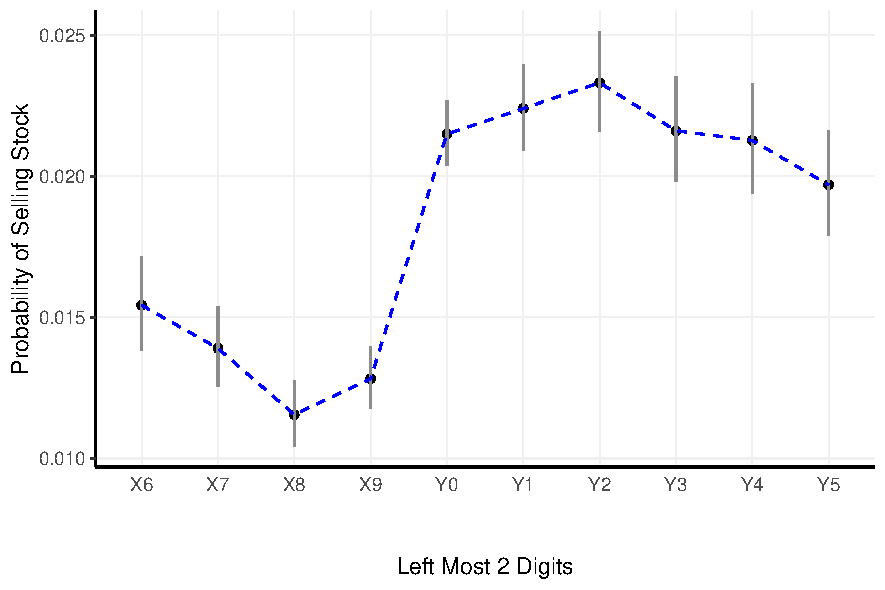
\includegraphics[width=0.45\textwidth]{figures/Left2increase_probCI2.pdf}
		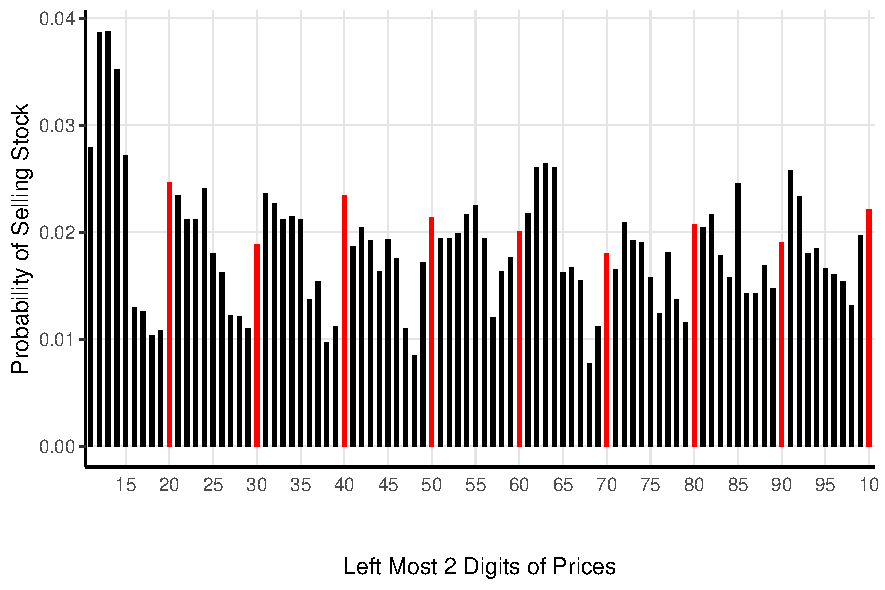
\includegraphics[width=0.45\textwidth]{figures/2left_increase2.pdf}	
	}
	\subfigure[Price Decreasing]{
		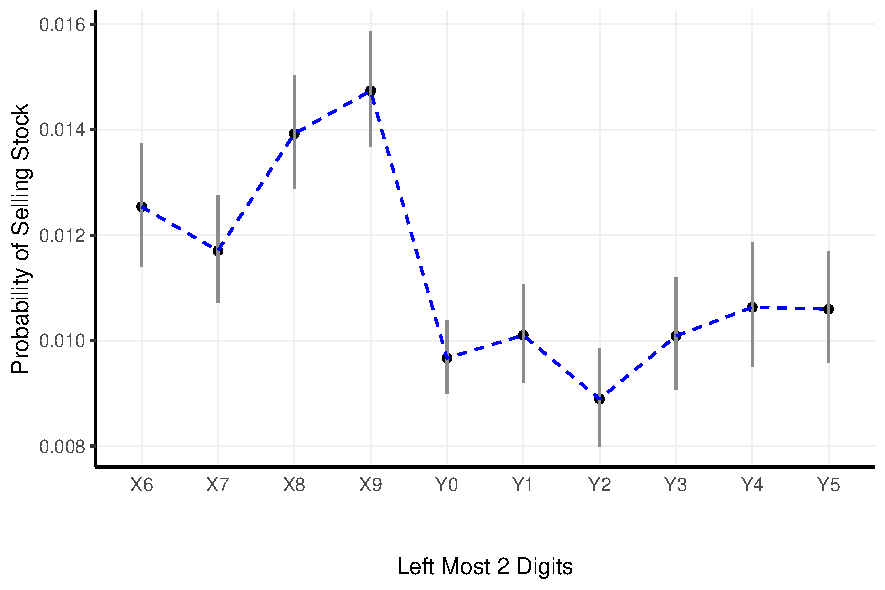
\includegraphics[width=0.45\textwidth]{figures/Left2decrease_probCI2.pdf}
		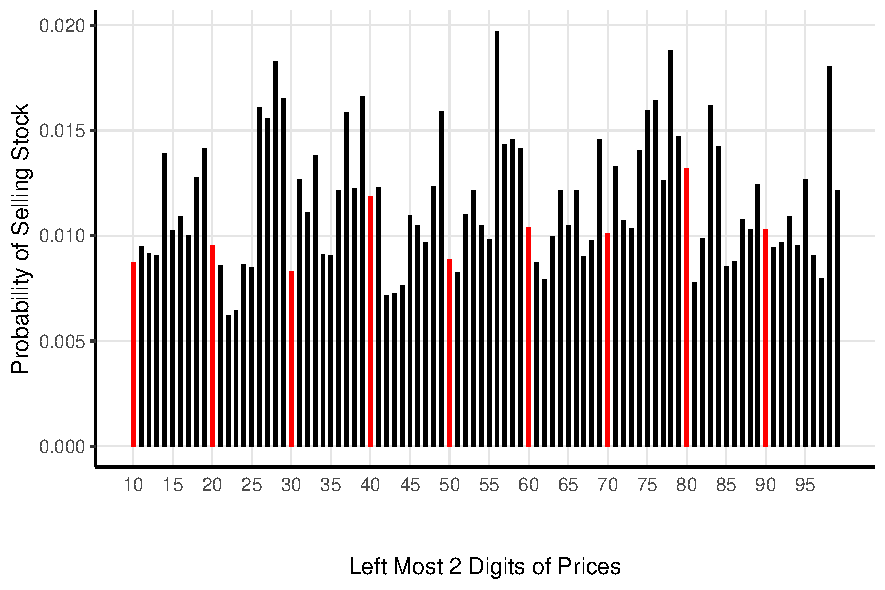
\includegraphics[width=0.45\textwidth]{figures/2left_decrease2.pdf}	
	}
	\fignote{£$Y$ in the X-axes is equivalent to £$X+1$ (e.g., £X9 could include £0.19, £1.9, £19, etc., while £Y0 could include £0.20, £2.0, £20, etc.).}
\end{figure}


